\documentclass[10pt,a4paper,titlepage]{report}
\usepackage{amsmath}
\usepackage{amsfonts}
\usepackage{amssymb}
\usepackage{fontspec}
\usepackage{graphicx}
\usepackage{tcolorbox}
\usepackage{lmodern}
\usepackage{xcolor}
\usepackage{listings}
\usepackage{color}
\usepackage{tikz}
\usepackage{pgfplots}
\pgfplotsset{compat=newest}
\usepackage[figuresleft]{rotating}
\usetikzlibrary{shapes,arrows,trees,snakes,patterns, decorations.markings,positioning,decorations.pathreplacing,plotmarks,calc, shapes, backgrounds}
\usetikzlibrary{intersections,positioning,arrows,calc,patterns,shapes.multipart,fit,backgrounds,decorations.pathreplacing}
\usepackage[final,backref=section,
bookmarks=true,
hypertexnames=true,
hyperindex=true,
hyperfootnotes=true,
linktocpage=false,
hyperfigures=true,
breaklinks=true,
pdfborder={0 0 0},
colorlinks=true,
linkcolor=black,
unicode=true,						
citecolor=blue,
urlcolor=blue,
pdfinfo={
	Title={Akkadian Word Segmentation Developers Documentation},
	Subject={Akkadian Word Segmentation Developers Documentation},
	Author={Timo Homburg},
	Keywords={Assyriology, Cuneiform, Akkadian, Chinese, Word Segmentation, Machine Learning}
}]{hyperref}
\definecolor{gray}{rgb}{0.4,0.4,0.4}
\definecolor{darkblue}{rgb}{0.0,0.0,0.6}
\definecolor{cyan}{rgb}{0.0,0.6,0.6}
\lstset{
	basicstyle=\footnotesize,
	frame=single,,
	columns=fullflexible,
	showstringspaces=false,
	commentstyle=\color{gray}\upshape,
	keepspaces
	% Linienstaerke des Rahmens
}

\lstdefinelanguage{XML}
{
	morestring=[b]",
	morestring=[s]{>}{<},
	morecomment=[s]{<?}{?>},
	stringstyle=\color{black},
	identifierstyle=\color{darkblue},
	keywordstyle=\color{cyan},
	morekeywords={xmlns,version,type}% list your attributes here
}
\setmainfont{Latin Modern Roman} %this is not needed as this should be the default
\setsansfont{Latin Modern Sans}
%\setmonofont{Andale Mono}

\newfontfamily\akkadian[AutoFakeBold,AutoFakeSlant]{Akkadian}
\newfontfamily\akkadiann[AutoFakeBold,AutoFakeSlant]{CuneiformNAOutline}
\newfontfamily\chinese{AR PL UKai CN}
\newfontfamily\japanese{IPAGothic}
\title{Akkadian Word Segmentation\\ Developers Documentation}

\author{Timo Homburg \\
	Institute for Computer Science\\
	Goethe University, Frankfurt, Germany \\
	{\tt timo.homburg@gmx.de}}
\begin{document}
	\maketitle
	\tableofcontents
	\ \\
	\chapter{Introduction}
	This document is the developer documentation of a Master thesis project for the prupose of segmenting Akkadian cuneiform texts. It will give a short introduction on how to use this application to segment texts and how to interpret results and how to extend the application.
	\section{Purpose}
	The purpose of the application can be described by describing its components:
	\begin{itemize}
		\item CorpusImportModule: Imports Corporadata
		\item CorpusHandlingModule: Prepares Corpora for classification purposes
		\item DictionaryModule: Collection of gained corpora data
		\item EvaluationModule: Evaluates generated segmentations by comparing them to the original segmentations
		\item SegmentationModule: Implements algorithms to segment
		\item TransliterationModule: Assigns transliterations to an already segmented text
		\item TranscriptionModule: Convertes transliterations to transcriptions
		\item POSTaggingModule: Tries to POSTag already texts in transliteration or Unicode representation
		\item TranslationModule: Using the POSTaggingModule tries to translate a given text to a given target language
		\item GUIModule: Displays statistics and Comparion Views 
	\end{itemize}
	This documentation will aim to explain every module and the corresponding classes and provide an idea for an developer on how to extend the program to fit the needs. Furthermore the intended naming scheme and resource files of the program shall be illustrated. It should also provide a guideline on how to use the program to classify different other languages than already implemented. 
	\chapter{Getting Started}
	In this chapter a brief introduction on how to start and work with the program shall be given. Before starting the program make sure a recent Java Virtual Machine Version 1.7 or higher is installed on your system.
	\section{How to use it}
	The program can be started using the following command: \begin{lstlisting}
	java -jar wordseg.jar
	\end{lstlisting}
	In this case, the graphical user interface will be started.\\
	Moreover the program offers the following options to work with it:
	\begin{itemize}
		\item Command Line interface for classifying data. This command line interface is currently not up-to-date.
		\begin{lstlisting}
		Main
		\end{lstlisting}
		\item Creation of FeatureSets using FeatureSet Generators with the following class:
		\begin{lstlisting}
		ArffHandler
		\end{lstlisting}
		\item Single execution of a classifier for Machine Learning to create models
		\begin{lstlisting}
		WekaMethods
		\end{lstlisting} 
	\end{itemize}
	\clearpage
	\subsection{Data structure}
	The program needs a certain data structure of folders to be started. The data structure is illustrated in the following figure:
	\begin{figure}[htb]
		\centering
		\tikzstyle{every node}=[draw=black,thick,anchor=west]
		\tikzstyle{selected}=[draw=red,fill=red!30]
		\tikzstyle{optional}=[dashed,fill=gray!50]
		\begin{tikzpicture}[%
		grow via three points={one child at (0.5,-0.7) and
			two children at (0.5,-0.7) and (0.5,-1.4)},
		edge from parent path={(\tikzparentnode.south) |- (\tikzchildnode.west)}]
		\node {root}
		child { node (dict) {dict} }
		child { node{ime}}
		child {node {pos} }		
		child { node [optional] {reformatted}
			child { node {boundary} }
			child { node {cuneiform}}
			child { node {cuneiform\_segmented}}
			child { node {translit}}
		}
		child [missing] {}				
		child [missing] {}				
		child [missing] {}
		child [missing] {}
		child {node [optional]{results}
			child { node {eval}}
			child { node {cuneiform}}
			child { node {translit}}
			child { node {transcript}}
			child { node {translation}}
		}				
		child [missing] {}				
		child [missing] {}
		child [missing] {}
		child [missing] {}
		child [missing] {}
		child { node {source}}				
		child { node {trainingdata}}
		child {node {testingdata}
		};
		\end{tikzpicture}
		\caption{Data and folder structure}
	\end{figure}
	\\The naming conventions of the program are as follows and will be illustrated further in the corresponding chapters:
	\begin{itemize}
		\item Preformatted corpora stick to their originally given name and are moved to the folder reformatted
		\item Resultfiles have the following naming scheme:
		\begin{lstlisting}
		sourceFileName_TestMethod_ClassificationMethod_TransliterationMethod_result.txt
		Zum Beispiel:
		corpus_crossvalidation_minwcmatch_first_result.txt
		\end{lstlisting}
		\item Statistics are named as follows:
		\begin{lstlisting}
		sourceFileName_TestMethod_ClassificationMethod_TransliterationMethod_eval.txt
		Zum Beispiel:
		corpus_crossvalidation_minwcmatch_first_eval.txt
		\end{lstlisting}
	\end{itemize}
	\section{Navigation and Options}
	Options to start a classification shall be presented as follows:
	\subsubsection{Classification}
	A classication chain needs the following parameters to be started:
	\begin{itemize}
		\item ClassificationMethod
		\item TransliterationMethod
		\item TranslationMethod
		\item Trainingfile
		\item Testfile
		\item TestMethod - Crossvalidation, Percentage Split...
		\item CharType - Which language?
		\item Target language
	\end{itemize}
	Every parameter can be in need of other parameters. For example: A featureset is needed if the classification method is a Machine Learning classifier.
	\subsubsection{Input Method Engine}
	Data for input method engines can be created for the following implementations:
	\begin{itemize}
		\item Ibus\footnote{Ibus: \href{https://code.google.com/p/ibus/}{https://code.google.com/p/ibus/}}
		\item JIMF (Java Input Method Framework)\footnote{JIMF: }
		\item JQuery: Für die Eigenentwicklung Webime\footnote{WebIME: \href{https://github.com/situx/webime}{https://github.com/situx/webime}}
		\item SCIM\footnote{SCIM: \href{http://sourceforge.net/projects/scim/}{http://sourceforge.net/projects/scim/}}
	\end{itemize}
	\subsubsection{Visualisation}
	The visualisation of the processing chain is described in chapter GUIModule. Every module contributing to the result of the will be presented with an own comparison and statistic view.
	\chapter{Structure}
	The structure of the program will shortly be outlined in this chapter. Modules mentioned in this package structured will later be presented in detail in the chapter Modules.
	The source code was designed to be able to cope with any language to be segmented. Another focus was to keep the code as extensible as possible.
	\section{Packages and Classes}
	The program was separated into the following packages:
	\begin{itemize}
		\item de.unifrankfurt.cs.acoli.akkad.dict
		\begin{itemize}
			\item de.unifrankfurt.cs.acoli.akkad.dict.chars - Definition of Character classes for different languages
			\item de.unifrankfurt.cs.acoli.akkad.dict.corpusimport - ImportHandler to import data from XML and ATF
			\item de.unifrankfurt.cs.acoli.akkad.dict.dictHandler - DictHanler to manage words and characters extracted from corpora
			\item de.unifrankfurt.cs.acoli.akkad.dict.importHandler - ImportHandler for previously exported dictionaries
			\item de.unifrankfurt.cs.acoli.akkad.dict.pos - POSTagger
			\item de.unifrankfurt.cs.acoli.akkad.dict.utils - Util classe for managing dictionaries
		\end{itemize}
		\item de.unifrankfurt.cs.acoli.akkad.eval - Evaluationmetrics and statistics
		\item de.unifrankfurt.cs.acoli.akkad.main - Graphical user interface and command line tools
		\item de.unifrankfurt.cs.acoli.akkad.methods - Segmentation, transliteration, transcription and translation methods
		\item de.unifrankfurt.cs.acoli.akkad.dict.util - Enums to store options
	\end{itemize}
	\section{Extensibility}
	To add another language the following steps need to be done:
	\begin{itemize}
		\item Define a character class and add its definition to the CharTypes Enums
		\item Define a DictHandler class
		\item Define a CorpusHandler class to handle imports of the corpus format
	\end{itemize}
	Upon creating support for a new language, all segmentation methods can be used on this new language instantly. If implemented correctly no further modifications are needed.
	As it concerns transliteration, transcription, POS-Tagging and translation, they have to be modified language dependently to fit the users needes.
	\chapter{Modules}
	\label{sec:modules}
	Modules provide the core functionality to the program. The presented modules work together to build a natural language processing chain illustrated in figure \ref{fig:pipeline}.
	\begin{figure}[htb]
		\tikzstyle{decision} = [diamond, draw, fill=blue!20, 
		text width=4.5em, text badly centered, node distance=3cm, inner sep=0pt]
		\tikzstyle{block} = [rectangle, draw, fill=blue!20, 
		text width=7em, text centered, rounded corners, minimum height=5em]
		\tikzstyle{line} = [draw, -latex']
		\tikzstyle{cloud} = [draw, ellipse,fill=red!20, node distance=3cm,minimum height=2em]
		\begin{tikzpicture}[node distance = 4cm, auto]
		% Place nodes
		\node [block] (start) {Text};
		\node [block, fill=blue!40,right of=start] (transformc) {Segmentation};
		\node [block, right of=transformc] (translit1) {Transliteration};
		\node [block, below of=translit1] (construct) {POS-Tagging};
		\node [block, left of=construct] (segment) {Grammar};
		\node [block, left of=segment] (translit2) {Translation};
		% Draw edges
		\path [line] (start) -- (transformc);
		\path [line] (transformc) -- (translit1);
		\path [line] (translit1) -- (construct);
		\path [line] (construct) -- (segment);
		\path [line] (segment) -- (translit2);
		\end{tikzpicture}
		\label{fig:pipeline}
		\caption{Natural Language Processing Pipeline as (partly) implemented in the program}
	\end{figure}
	\\ In its current state the focus was to implement the segmentation part of the chain. The implementation of other parts has begun but very often can be considered as rudimentary at this state. More information about the current status will be provided in the corresponding subsections of the modules.
	
	\section{CorpusHandlingModule}
	The corpus handling module manages the import of a corpus, its transformation in to an annotated dictionary and a classification task performed on the corpus using a predefined classification method. In particular the following corpus modes are supported:
	\begin{itemize}
		\item Manual selection of a Trainingfile and a Testfile
		\item Crossvalidation on the corpus (Fold can be specified)
		\item Percentage Split on the corpus (Percentage can be specified) on a char or text basis
		\item Random Split on the corpus (Percentage and text or char based randomness can be specified)
	\end{itemize}
	If a mode is chosen, the corpus handling module proceeds as follows:
	\begin{enumerate}
		\item Split the corpus according to the needs of the method
		\item Save splitted files for further use
		\item Start a classification task
	\end{enumerate}
	To implement a new corpus splitting method, this method needs to be registered in the corresponding Enum \textit{TestMethod}.
	Next, the proposed method needs to be implemented in the class \textit{CorpusHandlerAPI}, the class of which every CorpusHandlerModule inherits or a class inheriting \textit{CorpusHandlerAPI}. Mostly splitting methods are not language dependent and can therefore be implemented in the class directly.
	\subsection{General Attributes}
	A CorpusHandlerAPI shall always convert the given texts to the reformatted version used by segmentation algorithms. This means it has to call an import handler to import text data and create a dictionary from the desired training part after the chosen splitting process and should over conversion methods to interact between various occuring formats:
	\begin{itemize}
		\item Conversion to boundary format
		\item Conversion from UTF8 to ASCII and vice versa
		\item Conversion from corpus data to intermediate format 
	\end{itemize}
	
	\subsection{CorpusImportModule}
	\label{sec:corpusImport}
	The corpus import module aims to import data from given corpora or dictionaries.
	To import a certain dictionary or corpus it is necessary to define an Importer class which has to inherit the abstract class \textit{ImportHandler}.
	The required methods by implementing this class are as follows:
	\begin{itemize}
		\item reformatToASCIITranscription 
		\item reformatToUnicodeTranscription
	\end{itemize}
	This is to provide support for transliterations using diacritic signs and ASCII transcriptions/transliterations replacing them with numbers.
	Results of the parsing process shall be imported into a DictHandler described in \ref{sec:dictionaryModule} to be further processed in the segmentation process. One should also be aware of the language to be parsed. If no language support classes have been developed in the DictionaryModule language processing cannot occur properly.
	\subsection{Special Import Needs}
	Some corpora are used to be exported as one corpus file, while many corpora versions are used to be shipped in files contained in several directories. 
	To accomodate those needs the CorpusHandlingModule needs to call the CorpusImportModule many times to merge its results. It is also possible to merge a many-file corpus format into a one-file corpus format to simplify processing of corpora.
	\section{DictionaryModule}
	\label{sec:dictionaryModule}
	The dictionary module is the core data management module of the application. Any corpus being analyzed and transferred into the program will be internally converted into a dictionary which may or may not be exported. To define a dictionary it is necessary to define the language of the dictionary first. As until now it is only possible to include single language corpora. 
	Any dictionary consists of a DictHandler, a managing class of the dictionary and a language or writing specific character class.
	\subsection{Character Classes}
	Character classes are multifunctional classes defining both characters and words as they appear in the corresponding language. They hereby consist of basic attributes described in the class \textit{LangChar}. Those attributes are attributes any character of a language can include e.g. \begin{itemize}
		\item Relative/Absolute Occurance of the character in a corpus
		\item List of Transliterations
		\item List of Translations
		\item Preceding/Following Chars with occurances
		\item Encountered POSTags
		\item Character length
	\end{itemize}
	If on a character basis the character length describes the number of bytes used to represent this character in Unicode. This might as well vary in between the same language (e.g. Chinese) depending on the unicode block and has therefore be annotated on a per-char basis.\\
	Character classes are dependent on an initial language configuration enum defined in \textit{CharTypes}. Within this enum the following language specific parameters need to be configured upon creating a new language:
	\begin{itemize}
		\item Enum Identifier
		\item Language Name to display in the graphical user interface
		\item Locale String (Java if available, otherwise costumized String)
		\item Char Length in Unicode (if many apply the most common char length)
		\item List of StopChars before and after which a segmentation has to occur
		\item Regular Expression to define legal transliteration characters
	\end{itemize}
	\subsubsection{Language Specific Character Classes}
	Language specific character classes like AkkadChar inherit LangChar. If a language uses a common writing system used by other languages it might be useful to include another layer of more generalized classes. For example the class CuneiChar works as the base class for the Cuneiform language classes AkkadianChar, SumerianChar and HittiteChar as all three languages are written in Cuneiform.
	Typical criteria on a language specific or writing specific level include:
	\begin{itemize}
		\item Grammar aspects such as: Determinatives and Sumerograms in Akkadian or Word Categories like Number, Name a.s.o. in Chinese
		\item Suffix, Prefix, Infix indicators
	\end{itemize}
	\subsection{DictHandler}
	A DictHandler is a managing class for managing corpus data already organised in a dictionary form. It contains statistical data, the words of the dictionary and several mappings between the components.
	Every DictHandler class inherits the abstract class DictHandling which provides the following basic methods for a DictHandler: 
	\begin{itemize}
		\item addWord/addFollowingWord/addPrecedingWord/addStopWord - Adding words with several functions to the dictionary
		\item calculateAvgWordLength - Calculates the average word length under consideration of the current char length
		\item matchWord/matchWordByTransliteration/matchWordByTranscription - Lookup methods for the dictionary
		\item parseDictFile - Imports an already preformatted dictionary
		\item toIME - Exports the dictionary to an IME representation as defined in the \textit{ExportMethods} Enum
	\end{itemize} 
	\subsection{New Dictionary}
	To create a new dictionary by using an already existing or costumized CorpusImportModule the following implementation steps have to be done:
	\begin{enumerate}
		\item Create a character class in de.unifrankfurt.cs.acoli.akkad.dict.chars and let it inherit from LangChar
		\item Implement potentially missing methods
		\item Implement a new class inherting DictHandling or one of its subclasses
	\end{enumerate}
	\subsection{Adding External Resources}
	External Resources can be added to a dictionary to enrich it. Preferred resources would be translations, POSTagging information or statistics. To import translations from Websites, a WebCrawler Module has been implemented in the class \textit{DictWebCrawler}.
	Importer for external resources can be found in the dictionary module. Those have to be manually started after parsing the dictionary. Examples are the classes \textit{TranslationImportHandler} and \textit{TranslationImportHandler2}.
	\section{EvaluationModule}
	\label{sec:evaluationModule}
	The Evaluation module evaluates given segmentations by comparing it to the original segmentation. It therefore offers to implement several algorithms for this purpose. Results of an Evaluation are stored in an \textit{EvalResult} object and can further be processed e.g. in the GUI module for graphs or tables. EvalResult objects are collected in an \textit{EvalStatistics} object present in the \textit{Evaluation} class used to manage the evaluation process.  Algorithms will work either on a segmented transliteration or a segmented target text whereas the latter is preferred. Nevertheless the choice between the two options can be established in the initialization method of the class \textit{Evaluation} handling evaluation methods. The configuration of which methods to use is handled using the \textit{EvaluationMethod} Enum in which Evaluation methods are registered. To register an evaluation method the following items are required:
	\begin{itemize}
		\item Enum Identifier
		\item Log Identifier (for Evaluation Results in text form)
		\item Full Name Identifier
		\item The Evaluation Result Type
	\end{itemize}
	The Evaluation Result Type is configured in the \textit{EvalResultType} Enum and may take one of the following values:
	\begin{itemize}
		\item FScore - A metric producing precision, recall and fscore
		\item OneScore - A metric producing exactly one score as a result
		\item TwoScore - A metric producing two results as a score
	\end{itemize}
	\subsection{Export}
	Every evaluation process produces an export file save in the directory results/eval/. The result file includes the statistics of the given evaluation. 
	\begin{lstlisting}[caption=Evaluation File]
	======================Evaluating: results/translit/corpus_maxmatch_first_result.txt===========================
	Transliteration Evaluation
	Matched: 19902.0
	Missed: 31586.0
	Exp. Correct Segmentations: 0.0
	Total: 51488.0
	Matches(%): 38.65366687383468
	Misses(%): 61.34633312616532
	Accuracy(%): 92.9017357727978
	Precision(%):83.49555294512501
	Recall(%): 100.0
	F-Measure(%): 91.00553294617953
	G-Measure(%): 91.37590105992116
	TruePositive: 19902.0
	FalsePositive: 3934.0
	TrueNegative: 31586.0
	FalseNegative: 0.0
	\end{lstlisting}
	\section{SegmentationModule}
	\label{sec:segmentationModule}
	The segmentation module handles the segmentation of a given text. For this purpose the module refers to a segmentation algorithm desscription in the ClassificationMethod Enum consisting of the following attributes: 
	\begin{itemize}
		\item Name of the classification method
		\item Short description of the classification method
		\item Printing label of the classification method
		\item FeatureSet indicator
		\item A framework indicator defined by the Options Enum \ref{sec:options}
	\end{itemize}
	\subsection{Segmentation Method Collectors}
	Segmentation methods can be gathered in segmentation method collector classes which inherit a segmentation method type specific interface containing segmentation methods and the base abstract class \textit{SegmentationMethods}. It might be useful to group segmentation methods by type in those classes. Implementation examples are given with the interface \textit{DictMethodAPI} and the class \textit{DictMethods}.
	Important methods in \textit{SegmentationMethods} include:
	\begin{itemize}
		\item assignTransliteration - assigns transliterations by transliteration method an given dictionary
		\item fileToBoundaries - gets a boundary representation of the current input file for Machine Learning purposes
	\end{itemize}
	Apart from important methods the class contains FileReader and FileWriter objects needed to read and write the corresponding files to be classified.
	\subsection{Segmentation Method Collector Implementations}
	A segmentation method collector implementation consists of an init method and two methods at a time for one implementation of a segmentation method. The init method initializes the segmentation by preparing reader and writer objects and choosing desired parameters for a segmentation. It is called by one of the public segmentation methods and internally calls one of the private segmentation methods of the same name. For example: A call to public avgWordlength would call the init method using the parameter AVG as defined in the ClassificationMethod Enum to initialize the call of the private method avgWordlength for execution. Segmentation methods produce a segmentation results in Unicode characters, a transliteration result, a transcription result and a translation result. To make sure such results are produced on implementing a new segmentation method the segmentation result can be transformed to transliteration by using the method assignTransliteration of \textit{SegmentationMethods}.
	\subsection{Segmentation Method Collectors for Machine Learning}
	If Machine Learning is approached in one or many of the segmentation methods of a collector the generation of the featuresets and the handling of word boundary files has to be considered in the init method. The structure of a segmentation method collector changes as follows:
	\begin{itemize}
		\item Check if a Training and Testsets have already been generated
		\item If not training and/or test set has been generated, use the selected FeatureSetGenerator \ref{sec:featuresetgenerator} to do so
	\end{itemize}
	After having generated and/or checked for needed FeatureSets, Machine Learning algorithms accessed by using external frameworks are usually implemented in a framework specific class like \textit{WekaMethods}. This class provides the execution of the Machine Learning algorithm using the specified Training and Testsets, if necessary preprocessing methods which may or may not be provided by the framework, saving of models and the interpretation of results by retransforming them back into a segmented text.
	For the two used Machine Learning Frameworks WEKA and MALLET, the following facts need to be considered:
	\begin{itemize}
		\item WEKA expects the so-called ARFF format in which it is recommended to use a string representation for word segmentation characteristica as ngrams are a popular feature to use
		\item If a preprocessing is needed, WEKA transforms FeatureSets into a StringToWordVector representation. This can not be done if a multi-instance classification is done like in a HMM case
		\item If preprocessed using a StringToWordVector, the Machine Learning files will be in a so-called Sparse ARFF format. It is therefore necessary to check the first column for class 1 as 0s will be ignored
		\item Further implementations are needed for different result formats
		\item MALLET provides a simple result format that won't change depending on the algorithm. A sparse format does not exist	
	\end{itemize}
	\section{FeatureSets}
	\label{sec:featureset}
	FeatureSets are needed for Machine Learning purposes and mostly need to be generated in advance to process a specific text using FeatureSetGenerators.
	\subsection{FeatureSet Generators}
	\label{sec:featuresetgenerator}
	A FeatureSet Generator is a class in which an algorithm containing rules to build a specific FeatureSet are implemented. The algorithm receives a preformatted text and produces depending on its initial parameters a Trainingset including the class to be classified or a Testingset lacking the class to be classified.\\
	FeatureSets are defined in the enum FeatureSets using the following parameters:
	\begin{itemize}
		\item Array of classes of the featureset
		\item Number of features
		\item Name of the featureset
		\item Char or Wordbased Featureset indicator
	\end{itemize}
	Once a Featureset is registered, a featureset generator class can be implemented to contain the actual code of creating the featureset out of a text. A FeatureSet Generator class consists of a FeatureSetManager linking to the generating methods and FeatureSet Generator Collector classes implementing the generation methods.
	A FeatureSetManager inherits from FeatureSetAPI providing it with the method getContext, a method which for every character in the original text according to the selected featureset produces a line for the desired FeatureSet.\\
	\subsection{Generating a FeatureSet}
	Generating a FeatureSet requires a managing class to read the source text file and to write the destined FeatureSet file. Depending on the desired file format for the chosen Machine Learning framework this might need different managing classes. For now the ArffHandler class handles the creation of .arff files used in WEKA and .mallet files used in the MALLET framework. Depending on an Options Parameter \ref{sec:options} the class decides which format to produce. Classes like ArffHandlers are usually used in Segmentation Collectors for Machine Learning to generate Featuresets on-the-fly if not available previous to classifying. A featureset is generated in the subfolder trainingdata using a unique name of the file to be classified. More about names provides the section \nameref{sec:namingconvs}.
	\section{Transliteration Module}
	\label{sec:translitModule}
	The Transliteration Module is responsible for assigning transliterations to an already presegmented text. It is therefore necessary for an algorithm to choose an appropriate transliteration among predefined criterias. Already implemented transliteration methods are:
	\begin{itemize}
		\item Choose Transliteration according to the first transliteration in the transliteration list for the current word/char as present in the dictionary (First Transliteration)
		\item Choose Transliteration according to the transliteration in the transliteration list for the current word/char as present in the dictionary with highest frequency in the corpus (MaxProb Transliteration)
		\item Choose a random transliteration out of the transliteration list (Random)
	\end{itemize}
	The algorithms are implemented in the package methods.transliterations, yet they are encapsulated in the corresponding DictHandler module where they are delegated to the actual Character class implementing the call. A transliteration method should therefore be registered in the corresponding transliteration enum and the aforementioned chain of classes should be implemented to register the new method. The actual implementation will be in the corresponding Character class.
	\section{Transcription Module}
	\label{sec:TranscritionModule}
	The transcription module aims to produce a transcription of a previously transliterated text. In Akkadian this is currently done by removing syllable separators and converting so-called sumerograms to the Akkadian writing forms. For every language trying to be processed in this program, a transcription ruleset can be generated by creating a class and/or method linked to TranscriptionMethods. In the future, a transcription method can be added in the \textit{CharTypes} enum to get a fixed method of transliterting characters. It might also be useful to let the user pick an appropriate transcription method as many could exist in a language to choose from.
	\section{POSTagging Module}
	\label{sec:POSTagModule}
	The POSTagging Module is not only a module but can be used as a standalone program on its own in a forked POSTagger project becoming available shortly. The POSTagger module aims to POSTag an already segmented and transliterated text to get information about the word types and to approach an evaluation of the given segmentation. The POSTagger is currently implemented in a simple rulebased manner. Rules can be defined using Regular Expressions and will be used by the postagger to classify texts. This is by far not an optimal solution and can not in all aspects be used in every language. Especially irregular languages would need an update of this module to a statistical approach.
	The rulebased POSTagging module consists of the following parts:
	\begin{itemize}
		\item POSDefinition Files
		\item Dictionary
		\item IME
	\end{itemize}
	\subsection{POSDefinition File}
	A POSDefinition file is an XML file containing definitions of POSTags and regular expressions to detect them. To discover attributes of already recognised word types a second stage allows to process those words to filter those criterias. 
	Listing \ref{postagfile} shows an example file of a POSDefinition:
	\begin{lstlisting}[caption=POSDefinition File\label{postagfile}]
	<colors>
	COLOR SECTION -> Colors for coloring the words according to word types are saved here
	<tagcolor tag="DEFAULT" desc="default" matchorder="13" color="#C0C0C0"/>
	<tagcolor tag="CARD" desc="number" matchorder="1" color="#FFC0CB"/>
	<tagcolor tag="PREP" desc="preposition" matchorder="2" color="#00FFFF"/>
	...
	</colors>
	<dependencies>
	DEPENDENCIES for grammars can be defined here
	<dependence dependee="PREP" depender="DET"/>
	<dependence dependee="DET" depender="PRO"/>
	...
	</dependencies>
	<groupconfigs>
	GROUPS define already recognized word types to gain further information about them
	<groupconfig tag="VV" desc="verb">
	<!-- (la/li/le/lu for past tense or ni for plural)
	(Vocal before first root)
	(Vocal after first root)
	(ta-,te- for Perfect) -->
	<group desc="verb" tag="VV" 
	name="Case:  First Person Plural" 
	regex="^(ni|nu)-$" group="2" case="declination" value="FIRST_PLURAL"/>
	<group desc="verb" tag="VV" 
	name="Tense: Past Tense" 
	regex="^(li|la|le|lu)-$" group="2" 
	case="tense" value="PAST" />
	</groupconfig>
	</groupconfigs>
	<tags>
	TAGS define word types and their corresponding Regular Expressions,
	Transliteration and Translation values if appropriate
	<tag desc="verb" name="VV"  
	equals="" regex="^.*(𒁕).*$" case="VERB" value="ta verb" />
	<tag desc="verb" name="VV"  
	equals="" regex="^.*(𒊹).*$" case="VERB" value="te verb" />	
	<tag desc="number" name="CARD" 
	equals="" regex="^(𒁹)+$" cunei="disz" case="NUMBER" value="1"/>
	<tag desc="pronoun" name="PRO" 
	cunei="a-na-ku-ma" equals="𒀀𒉌𒆪𒈠" regex="" 
	case="FIRST_SINGULAR_NOMINATIVE" value="I" />
	<tag desc="nounoradj" name="NA" equals=""
	regex="(.*(-sza))$" case="FIRST_GENITIVE_SINGULAR_FEMALE"/>
	<tag desc="nounoradj" name="NA" equals=""
	regex="(.*(-szi))$" case="FIRST_ACCUSATIVE_SINGULAR_FEMALE"/>
	\end{lstlisting}
	POSDefinition files are stored in the folder pos/ and are usually named after the language shortcut they are implementing. The language shortcut has to be defined in the corresponding CharTypes enum in the program.
	\begin{figure}[htb]
		\centering
		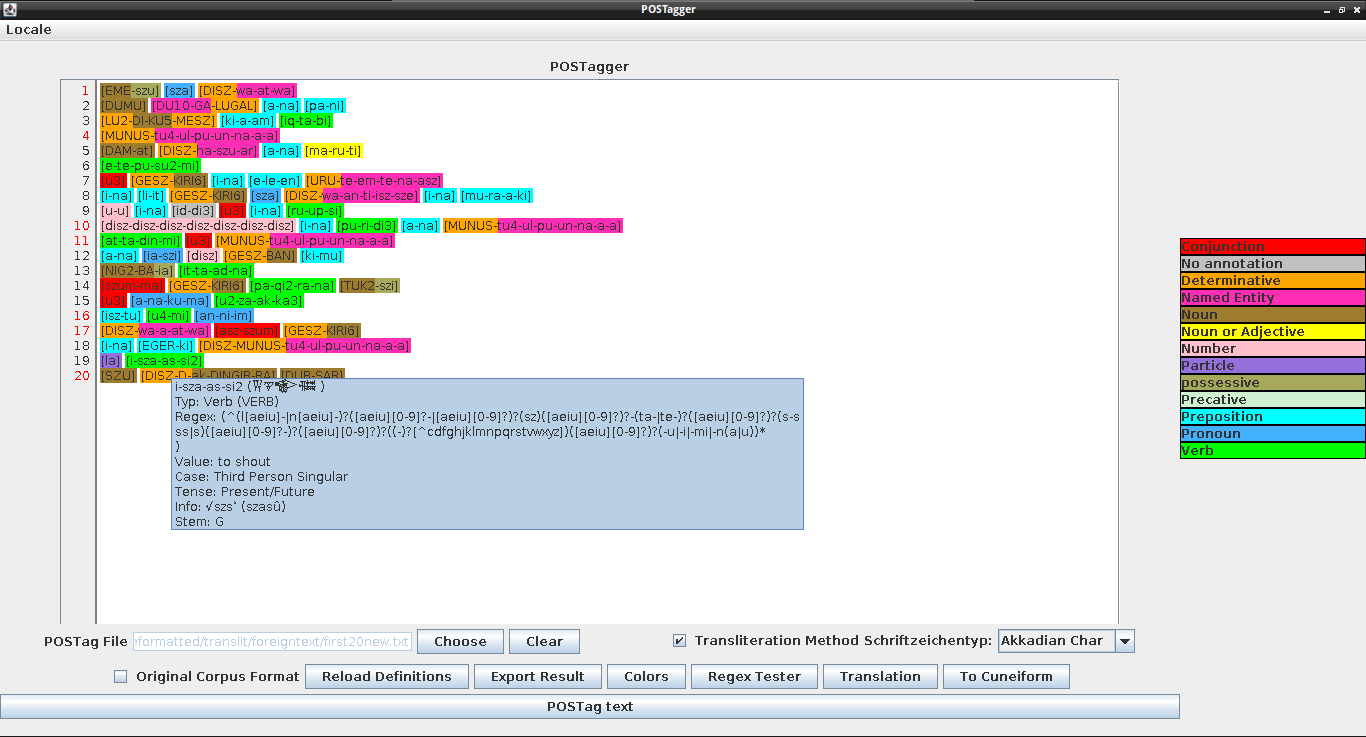
\includegraphics[width=1\textwidth]{images/postagging.png}
		\caption{External POSTagging Example}
		\label{fig:postagging}
	\end{figure}
	\subsection{Dictionary}
	If integrated into the main program the POSTagger can use the dictionaries the main program is using. If exported to an extra application those dictionaries have to be transferred as well.
	\subsection{IME}
	An unfinished approach let the POSTagging module use an Input Method Enging for Akkadian to input text that is on-the-fly classified by methods of POS-Tagging. This is a feature only present in the standalone version and ist not intended for the word segmentation tool. However an input method engine can be tested in one of the option selections. More about Input Method Engines is provided in the corresponding section.
	\section{Translation Module}
	The translation module can also be used in the standalone version of the POSTagging module and therefore has to applications. If used in the segmentation program it will try a plane 1:1 word translation if the word given is recognised. This is not yet very effective as word types and forms are not considered. In the external POSTagger program at first  POSTagging is generated on the given text and then according to the given translation information through external resources the algorithm tries to produce an enhanced word-by-word translation considering word forms.
	\begin{figure}[htb]
		\centering
		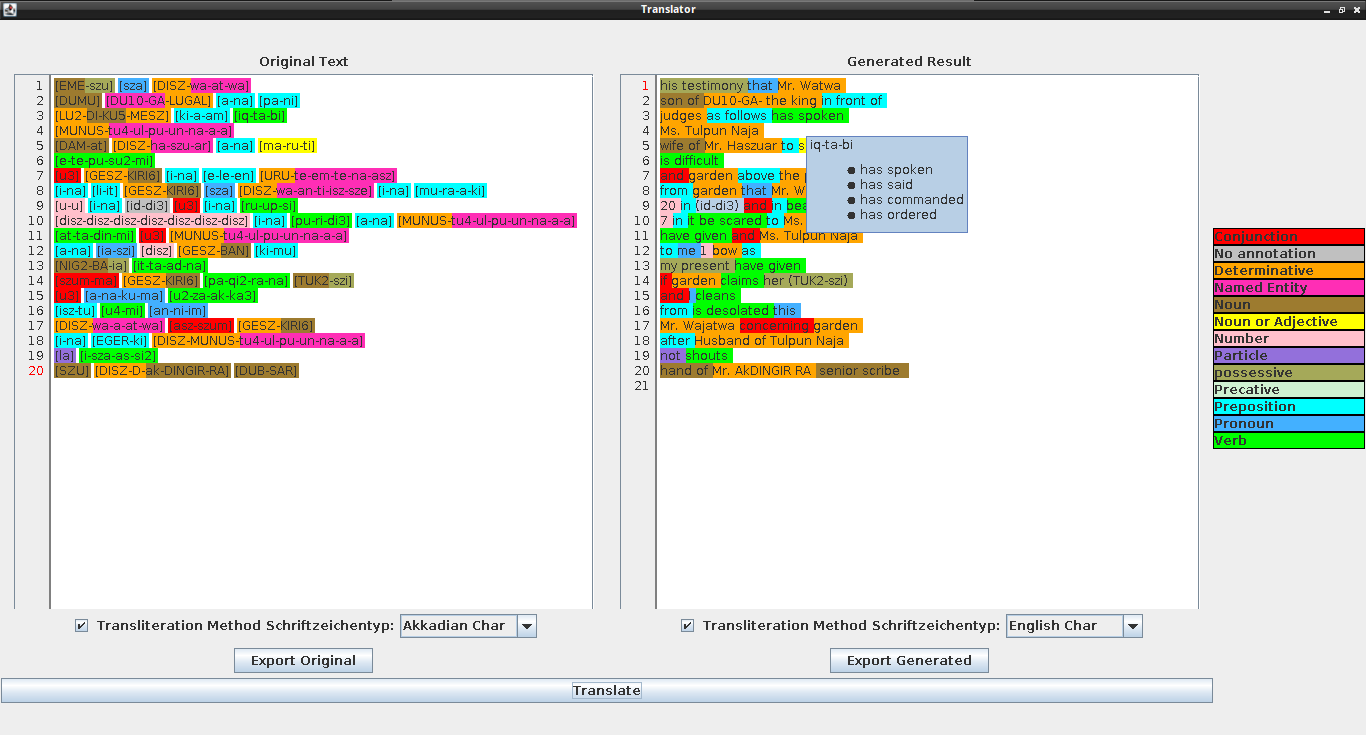
\includegraphics[width=1\textwidth]{images/translation.png}
		\caption{External Translation Example}
		\label{fig:translation}
	\end{figure}
	\subsection{Translator Classes}
	To perform a translation one has to define a source language and a target language.
	\section{GUIModule}
	\label{sec:guiModule}
	The GUI module is defined in the package main.gui. It contains a starting screen, a statistic screen, several comparison screens and a few option screens.
	\subsection{Internationalization}
	The program supports Java Resource Bundles common in many Java Applications. However the class to load Resource Bundles needed to be rewritten to confirm to an UTF-8 Loading behavior of ResourceBundles. The implementation is located in the class \textbf{UTF-8 Bundle}. So far an English and German localization with English being the default have been implemented. Further support of languages is appreciated.
	\subsection{Title Screen}
	The title screen is where the user is able to choose the desired algorithm among other configurations (see Figure \ref{fig:advgui})
	\begin{figure}[htb]
		\centering
		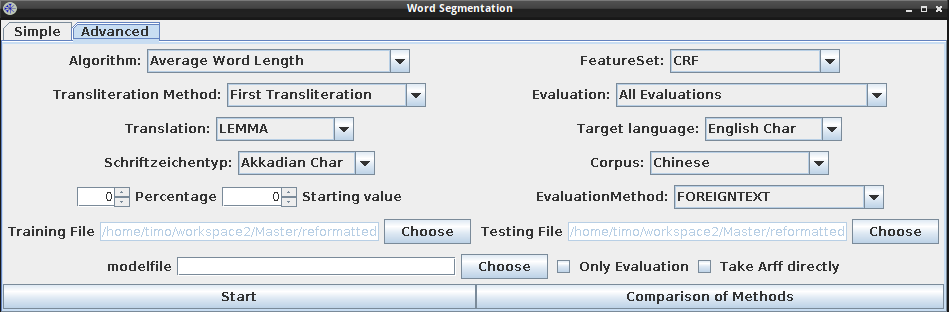
\includegraphics[width=0.8\textwidth]{images/advgui.png}
		\caption{Advanced GUI Screen}
		\label{fig:advgui}
	\end{figure}
	\\
	The starting screen is defined in the class MainGUI whereas \textit{MainGUI} inherits the \textit{GUIFormat} class defining a unified layout for all windows of the program. Calls from this view will be received by the class \textit{Main} which routes calls from the Graphical User Interface to the destined segmentation method classes described in \ref{sec:segmentationModule} \nameref{sec:segmentationModule}. 
	The implementation of the title screen has been refined to include a simple mode and an advanced mode. The simple mode was designed to offer simple algorithms which in a standard bundle of this application should work out-of-the-box and in a reasonable time. This makes the view a suitable one for presentations of the program. The advanced module was designed to offer all possibilities of the program as well as to begin Machine Learning training and similar longterm projects.
	\subsection{Comparison Screen}
	Comparison Screens are needed if comparisons between an original text and a segmented text should be presented to the user. The user should be able to see differences clearly and be able to find weaknesses of the implementations easily.\\
	\begin{figure}[htb]
		\centering
		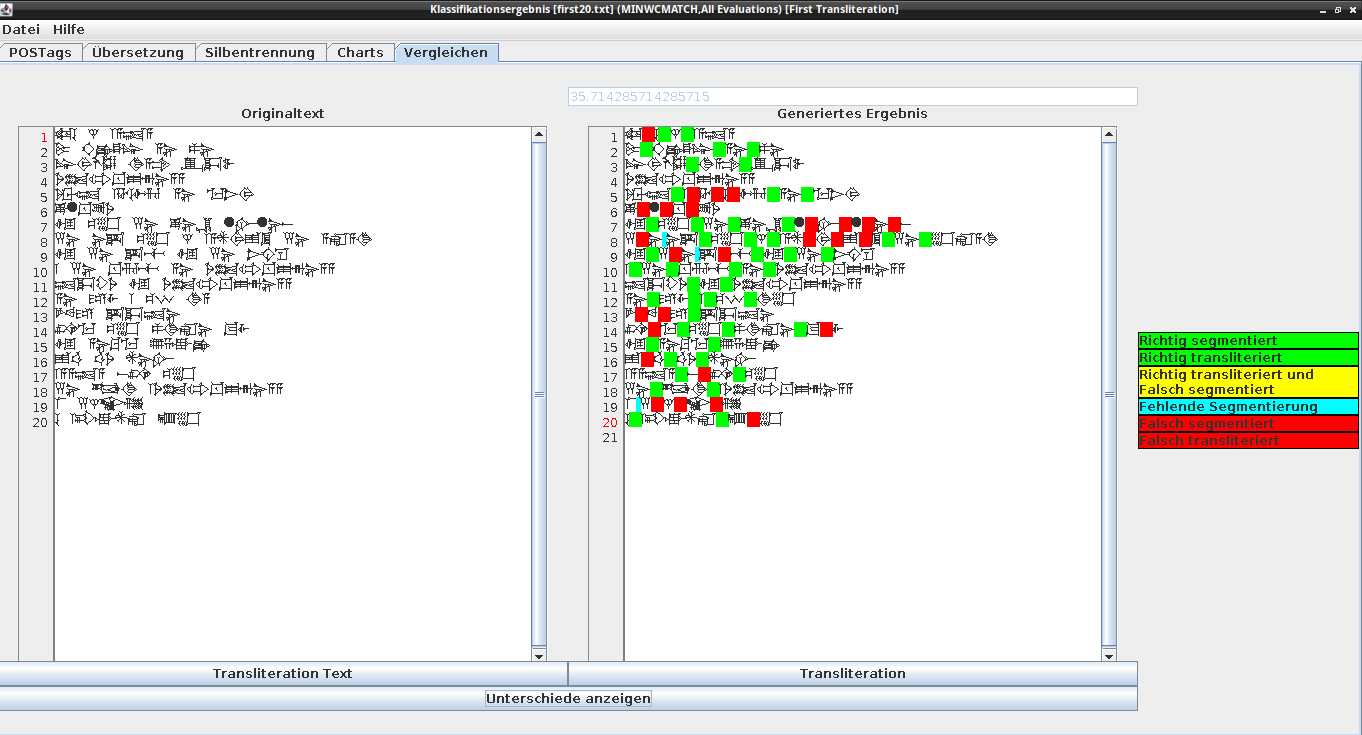
\includegraphics[width=1\textwidth]{images/comp.png}
		\caption{Segmentation Comparison Screen}
		\label{fig:comp}
	\end{figure}
	Comparison screens are used to 
	\begin{itemize}
		\item Compare Segmentations
		\item Compare Transliterations
		\item Compare Transliterations to Transcriptions
		\item Compare Original Texts to Translations
	\end{itemize}
	Every Comparison Screen inherits the abstract class \textit{CompGUI}.  This class implements the basic view of the window. A comparison window consists of two buttons, a legend and two JToolTipAreas, a costumized class to fit the needs of comparisons better. To highlight possible differences between segmentations JToolTipAreas will be colored using a highlighter. They may as well contain additional information depending on the screen.
	\begin{tcolorbox}[title=Implementation Advice]
		The implemented highlighting algorithms expect a whitespace after every word of text. This is implementation specific and also requires a whitespace in front of every newline. If a whitespace in front of a newline is missing the marking algorithm will produce malicious results.
	\end{tcolorbox}
	In some screens the legend should also be used as a tool to costumize the highlights given in the textareas. A map from whitespace to color should remember which spaces have been marked in which color to clear those spaces and redraw them if chosen in the legend respectively.
	\subsubsection{JToolTipArea}
	A JToolTipArea is a modified JEditorPane of Java Swing. It essentially contains the implementation of a Tooltip extension making it possible to display highlighting Tooltips over words. It also provides the option to directly copy a clicked word to the clipboard in order to conveniently copy selected texts. JToolTipAreas in itself also provide the data management for the given texts and annotations they contain and access methods respectively. JToolTipAreas also incorporate a sidebar in which the linenumbers are counted. In the case of the POSTagging module this sidebar also functions as a sentence end indicator using colored numbers and as a method to select sentences.
	\subsection{Statistics Screen}
	The statistics screen gathers information provided by the classes described in \ref{sec:evaluationModule}. 
	Information is usually represented in JTables and a graph is represented using the library JFreeChart.
	\subsubsection{Result Tables}
	Result Tables use modified TableRenderer structure which can be found in the untility pacage of the gui package. Inserted data from the evaluation classes will be considered and colored in a scale ranging from red to green. The coloring is performed on a scale from 0\% (red) to 100\% (green). Depending on the measure being used it might be suitable to create different TableRenderers to fit the needs to different measures.
	\subsubsection{Graph}
	The graph of the statistics screen was created using JFreeChart. In includes the Accuracy, Recall, Precision, F-Score and G-Scores of the different measures. If a measure does not contain the aforementioned measure it will be represented using the value 0 in all of them. It is therefore not a good idea to put single value measures in the graph as there is no room for comparison to an F-Score measure. However another JFreeChart graph could be used to incorporate single value measure in the future. To create a JFreeChart XYSeries of data have to be generated as an input format to the JFreeChart library. Result data from EvaluationResults have therefore to be processed further.
	\section{Utilities}
	\label{sec:utilities}
	In this chapter used libraries, utility classes and further applications of the programm shall be illustrated.
	\subsection{Libraries}
	\label{sec:libraries}
	The program uses the following libraries for the following purposes:
	\begin{table}[htb]
		\centering
		\begin{tabular}{|c|c|c|}
			\hline
			Library & License & Usage  \\
			\hline
			Abego Treelayout \footnote{\href{http://netbeans.dzone.com/efficient-and-customizable-java-treelayout}{http://netbeans.dzone.com/efficient-and-customizable-java-treelayout}  by Udo Borkowski} & BSD License & Treelayout classes to display syntactic trees\\
			\hline
			Apache Xerces\footnote{\href{http://xerces.apache.org/}{http://xerces.apache.org/} - Apache Xerces} & Apache License 2.0 & XML Parser\\
			\hline
			HMMWeka\footnote{\href{http://www.doc.gold.ac.uk/~mas02mg/software/hmmweka/index.html}{http://www.doc.gold.ac.uk/~mas02mg/software/hmmweka/index.html} - HMMWeka Plugin} & GPL & HMM Classifier as WEKA Plugin\\
			\hline
			Jericho HTML Parser\footnote{\href{http://jericho.htmlparser.net/docs/index.html}{http://jericho.htmlparser.net/docs/index.html} - Jericho HTML Parser} & LGPL & HTML Parser\\
			\hline
			JFreeChart\footnote{\href{http://www.jfree.org/jfreechart/}{http://www.jfree.org/jfreechart/} - LibSVM} & LGPL & Graph library\\
			\hline
			LibSVM\footnote{\href{http://www.csie.ntu.edu.tw/~cjlin/libsvm/}{http://www.csie.ntu.edu.tw/~cjlin/libsvm/} - LibSVM} & BSD License & SVM Classifier in WEKA Classifier\\
			\hline
			MALLET\footnote{\href{		http://mallet.cs.umass.edu/}{		http://mallet.cs.umass.edu/} - MALLET} & CPL 1.0 & MALLET CRF Classifier\\
			\hline
			Pig Latin IME Java \footnote{\href{http://jan.newmarch.name/i18n/input/input.html}{http://jan.newmarch.name/i18n/input/input.html}} & Creative Commons License & Creation of an Input Method Engine\\
			\hline
			Regular expression Tester \footnote{\href{https://www.cis.upenn.edu/~matuszek/General/RegexTester/regex-tester.html}{https://www.cis.upenn.edu/~matuszek/General/RegexTester/regex-tester.html}  by David Matuszek} & No restriction & Tester for Regular Expressions\\
			\hline
			SimpleNLG \footnote{\href{https://code.google.com/p/simplenlg/}{https://code.google.com/p/simplenlg/} (24.2.2015)} & Mozilla Public License 1.1 & Verb Generator\\
			\hline
			TextLineNumber \footnote{\href{https://tips4java.wordpress.com/2009/05/23/text-component-line-number/}{https://tips4java.wordpress.com/2009/05/23/text-component-line-number/}} & No restriction & LineNumber Panel\\
			\hline
			WEKA\footnote{\href{http://www.cs.waikato.ac.nz/ml/weka/}{http://www.cs.waikato.ac.nz/ml/weka/} - Waikato Environment for Knowledge Analysis} & GPL & kNN, kMeans, Logistic,\\
			& & MultiLayerPerceptron, NaiveBayes Classifier\\
			\hline
		\end{tabular}
		\caption{Libraries used in the program}
		\label{tab:libraries}
	\end{table}
	\subsection{Options}
	\label{sec:options}
	The options enum represents options that are needed throughout the program. Options may for example be the following facts: 
	\begin{itemize}
		\item Framework Names
		\item Training/Testingset Indicators
	\end{itemize}
	\chapter{Resources and Data}
	\label{sec:resourceData}
	This chapter is about the several resources and data formats used in the program as well as about its naming conventions to identify corresponding files.
	\section{Naming Conventions}
	\label{sec:namingconvs}
	Names of corpora depend on the names given to the corpora files when first given into the program. During the processing of corpus files the following files using the following naming conventions might be created:
	\subsection{Preprocessing}
	Corpus files will be preprocessed in various was in the subfolder reformatted consisting of 
	\begin{itemize}
		\item Transliteration (translit/)
		\item Boundary Representation (boundary/)
		\item Segmented Target Text (cuneiform\_segmented/)
		\item Unsegmented Target Text (cuneiform/)
	\end{itemize}
	Depending on which corpus segmentation method of the CorpusHandling Module was chosen several subfolders will be contained in the folders mentioned above:
	\begin{itemize}
		\item (Foreigntext/) - No special treatment of the text
		\item (Crossvalidation/) - Corpus text is splitted according to crossvalidation rules
		\item (Percentage/) - Corpus has been splitted according to a percentage split rule
		\item (RandomSample/) - A random sample of a corpus has been chosen
	\end{itemize}
	Files created in the above mentioned dictionaries will have the following name conventions:
	\begin{itemize}
		\item Name of the original file in source/
		\item If Crossvalidation it will append a suffix \_(NUMBER Of Split)
		\item If Percentage Split it will append a suffix \_t(PERCENT)
		\item If Random it will append a suffix \_t(PERCENT)
	\end{itemize}
	It is therefore feasible for the program to access files according to the corpus split method being selected.
	\subsection{FeatureSets}
	Using preprocessed data the program is able to create FeatureSets needed for Machine Learning. Machine Learning Data will be stored in the following folders: 
	\begin{itemize}
		\item trainingdata/ for Trainingsets
		\item testdata/ for Testsets
		\item trainingsdata/model for generated model files
	\end{itemize}
	The naming conventions for FeatureSets when generated by the program are as follows:
	\begin{itemize}
		\item Name of the reformatted file
		\item \_Name of the featureset as defined in the enum \textit{FeatureSets}
		\item File extensions according to the Machine Learning Framework
	\end{itemize}
	The program can therefore access the desired files by concatenating the source file name, the preprocessing step, the featureset name and the Machine Learning framework.
	\subsubsection{Model files}
	Model files represent already trained data and have therefore already been processed by a Machine Learning algorithm. The naming scheme therefore has to incorporate the Machine Learning algorithm to uniquely identify the model file.
	\begin{itemize}
		\item Name of the reformatted file
		\item Name of the algorithm used for training
		\item \_Name of the featureset as defined in the enum \textit{FeatureSets}
		\item File extensions according to the Machine Learning Framework
	\end{itemize}
	\subsection{Results}
	Results of the algorithm have to be saved in the folder results/. Within those folders various results can occur:
	\begin{itemize}
		\item Target language results (cuneiform/)
		\item Evaluation statistics (eval/)
		\item Transliteration results (translit/)
		\item Transcription results (transcript/)
		\item Translation results (translartion/)
	\end{itemize}
	A result file consists of all the elements necessary to create the result file namely:
	\begin{itemize}
		\item Name of the reformatted file	
		\item \_Segmentation Method
		\item Optional: \_Name of the featureset as defined in the enum \textit{FeatureSets}
		\item \_Transliteration Method
		\item Suffix \_result
	\end{itemize}
	\section{Corpora Data}
	Resources consist of corpora data stored in different formats and are usually stored in the subfolder source.
	Names of the corpora data can be freely choosen but will become possible unique identifiers for further classifications.
	Examples of corpora data can be the ATF-Format for cuneiform:
	\begin{lstlisting}[caption=ATF-Format as Corpus Format]
	&P388494 = AASOR 16, 015
	#atf: lang akk
	@tablet
	@obverse
	1. _eme_-szu sza {disz}wa-at-wa
	2. _dumu du10-ga-lugal_ a-na pa-ni
	3. {lu2}_di-ku5_{mesz} ki-a-am iq-ta-bi
	4. {munus}tu4-ul-pu-un-na-a-a
	5. _dam_-at {disz}ha-szu-ar a-na ma-ru-ti
	6. e-te-pu-us-su2-mi
	7. u3 {gesz}_kiri6_ i-na e-le-en {uru}te-em-<te>-na-asz
	8. i-na li-it {gesz}_kiri6_ sza {disz}wa-an-ti-isz-sze i-na mu-ra-a-ki
	9. 2(u) i-na szi2-id-di3 u3 i-na ru-up-szi#
	10. 7(disz) i-na pu-ri-di3 a-na {munus}tu4-ul-pu-un-na-a-a
	11. at-ta-din-mi u3 {munus}tu4-ul-pu-un-[na]-a-a
	12. a-na ia-szi 1(disz) {gesz}_ban_ ki-mu
	13. _nig2-ba_-ia it-ta-ad-na
	14. szum-ma {gesz}_kiri6_ pa-qi2-ra-na _tuk2_-szi
	15. u3 a-na-ku-ma u2-za-ak-ka3
	16. isz-tu u4-mi an-ni-im
	17. {disz}wa#-a-at-wa asz-szum {gesz}_kiri6_
	18. i-[na] _eger_-ki {disz}{munus}tu4-ul-pu-un-na-a-a
	19. la i-sza-as-si2
	\end{lstlisting}
	\section{Intermediate Format}
	The intermediate format is a special format used for segmentation purposes. The transliteration of a corpus is represented in syllables separated by the minus character and words enclosed in brackets separated by whitespaces. This format is language independent as every language should be able to be transformed in a format of this kind.\\
	Language dependent formats like 
	\begin{itemize}
		\item Segmented or unsegmented text of the target language
		\item Boundary representation of the text
	\end{itemize}
	can be generated from the intermediate format.
	\begin{lstlisting}[caption=Intermediate Format]
	&P388494 = AASOR 16, 015
	#atf: lang akk
	@tablet
	@obverse
	1. _eme_-szu sza {disz}wa-at-wa
	2. _dumu du10-ga-lugal_ a-na pa-ni
	3. {lu2}_di-ku5_{mesz} ki-a-am iq-ta-bi
	4. {munus}tu4-ul-pu-un-na-a-a
	5. _dam_-at {disz}ha-szu-ar a-na ma-ru-ti
	
	is transformed to the intermediate format:
	
	[eme-szu] [sza] [disz-wa-at-wa] 
	[dumu] [du10-ga-lugal] [a-na] [pa-ni] 
	[lu2-di-ku5-mesz] [ki-a-am] [iq-ta-bi] 
	[munus-tu4-ul-pu-un-na-a-a] 
	[dam-at] [disz-ha-szu-ar] [a-na] [ma-ru-ti] 
	\end{lstlisting}
	\section{Boundary Format}
	The boundary format is a representation used for Machine Learning. The given text in intermediate format is hereby transformed using the following rules:
	\begin{itemize}
		\item If the current syllable does not end a word write \textit{0,}
		\item If the current syllable ends a word write \textit{1,}
		\item Transfer newlines from the text into the new text
	\end{itemize}
	The result will be a boundary representation representing the necessary information of where a segmentation took place in the classes 0 and 1 for segmenting and not segmenting.
	\begin{lstlisting}[caption=Boundary Representation]
	[eme-szu] [sza] [disz-wa-at-wa] 
	[dumu] [du10-ga-lugal] [a-na] [pa-ni] 
	[lu2-di-ku5-mesz] [ki-a-am] [iq-ta-bi] 
	[munus-tu4-ul-pu-un-na-a-a] 
	[dam-at] [disz-ha-szu-ar] [a-na] [ma-ru-ti] 
	[e-te-pu-us-su2-mi]
	
	is transformed to the boundary representation:
	
	0,1,1,0,0,0,1,
	1,0,0,1,0,1,0,1,
	0,0,0,1,0,0,1,0,0,1,
	0,0,0,0,0,0,0,1,
	0,1,0,0,0,1,0,1,0,0,1,
	\end{lstlisting}
	\section{Target Language Formats}
	Target language formats represent text in the target language on which a segmentation should occur. Target language formats often require a manual or automated conversion process from the intermediate format using a list. Those resources can either be generated from corpora data directly or are delivered in the application root itself. For Akkadian, the file akkadian.xml represents such a table file.
	\begin{lstlisting}[caption=Target Language Representation,escapechar=!]
	[eme-szu] [sza] [disz-wa-at-wa] 
	[dumu] [du10-ga-lugal] [a-na] [pa-ni] 
	[lu2-di-ku5-mesz] [ki-a-am] [iq-ta-bi] 
	[munus-tu4-ul-pu-un-na-a-a] 
	[dam-at] [disz-ha-szu-ar] [a-na] [ma-ru-ti] 
	[e-te-pu-us-su2-mi]
	
	is transferred to the target language representation:
	
	!{\akkadian 𒅴𒋙 𒐼 𒁹𒀀𒀜𒀀}!
	!{\akkadian 𒌉 𒄭𒂵𒈗 𒀀𒉌 𒉺𒉌}!
	!{\akkadian 𒇽𒁲𒋻𒌊 𒆠𒀀𒄠 𒅅𒁕𒉿}!
	!{\akkadian 𒊩𒌅𒌌𒇥𒌦𒉌𒀀𒀀}!
	!{\akkadian 𒁮𒀜 𒁹𒄩𒋙𒅈 𒀀𒉌 𒈠𒆕𒁲}!
	!{\akkadian 𒂊𒊹𒇥𒍪𒊩}! 
	\end{lstlisting}
	\section{Dictionary Resources}
	Dictionary resources are located in the subfolder dict/ of the application. Dictionary resources are hereby defined as dictionaries created by the application itself. Those dictionaries can be considered as an import file format for corpora not requiring any resource files to be manually processed. They might as well be an XML solution for other programs.\\
	Dictionary resources are separated in \_map files and \_dict files. While map files only contain character mappings of a corpus, dict mappings can contain words and single characters if occured as words. Both files will be processed by the program according to the language enum. If the current language present is Akkadian the program will therefore search for the file dicts/Akkadian\_map.xml and dicts/Akkadian\_dict.xml.
	\subsection{Content}
	Dictionaries contain character to unicode mappings, characters statistics, transliterations, translations and POSTags as well as following and preceding words/chars with their corresponding statistics.
	\begin{lstlisting}[caption=Dictionary Contents,escapechar=!]
	<dictentry logogram="!{\akkadian 𒀀𒀀𒁕}!" determinative="false" logograph="false" phonogram="false" 
	relativeOccurance="1.2692656391659113E-4"
	absoluteOccurance="7.0" begin="0.0" middle="0.0" end="0.0" single="false">
	<transliteration begin="0.0" middle="0.0" end="0.0" single="0.0" isWord="false" 
	absoluteOccurance="1"
	relativeOccurance="1.813236627379873E-5">a-a-ta</transliteration>
	<following absoluteOccurance="2.0" absboundary="0.0">!{\akkadian 𒀭𒉌𒁕}!</following>
	<following absoluteOccurance="1.0" absboundary="0.0">!{\akkadian 𒆏𒉺}!</following>
	<following absoluteOccurance="1.0" absboundary="0.0">!{\akkadian 𒉌𒊑𒋙𒈿}!</following>
	<following absoluteOccurance="1.0" absboundary="0.0">!{\akkadian 𒍝𒇥𒌨𒁕}!</following>
	<following absoluteOccurance="1.0" absboundary="0.0">!{\akkadian 𒐼𒀀}!</following>
	!{\akkadian 𒀀𒀀𒁕}!</dictentry>
	\end{lstlisting}  
	\section{Exports}
	\label{sec:exports}
	The program features several exports from corpora data which should be highlighted in this section. The following exports opportunities exist:
	\begin{itemize}
		\item Input Method Engine Exports in folder (ime/):\begin{itemize}
			\item Ibus Input Method Engine (ibus\_header and ibus\_footer files needed to process)
			\item JQuery (jquery\_header and jquery\_footer files needed to process)
			\item SCIM (scim\_header and scim\_footer files needed to process)
		\end{itemize}
		\item Anki Export:
	\end{itemize}
	\section{Results}
	Results are stored in the subdirectory results/ and contain results for different purposes:
	\subsection{Boundaries}
	Boundary results are usually not stored in the program. Instead boundary results are retransformed into a target language or transliteration representation to simplify the evaluation process. The retransformation works as follows:
	\begin{itemize}
		\item According to the Machine Learning result try to parse the classification result per char
		\item Take a copy of the unsegmented target language text and on-the-fly enter whitespaces where the classification signifies
		\item Assign a transliteration to the result and continue in the natural language processing pipeline
	\end{itemize}
	In the end the result of boundaries becomes obsolete and is not saved in one of the subdirectories of results/.
	\subsection{Evaluation}
	For every evaluation taken place an evaluation file is saved in results/eval.
	\subsection{Target Language}
	A target language for the classification can be chosen in the application and will determine if the classification is done with e.g. an Akkadian, Hittite or Sumerian corpus. In fact, additional target languages can be defined in the program and can be used if corpora resources are available in the source/ directory.
	\subsection{Transliteration}
	Transliteration files are saved in folder reformatted/translit. According to the transliteration method chosen and the configuration of the classification they will be placed in a subdirectory of transliteration according to the split of the corpus.
	\subsection{Transcription}
Transcriptions are generated from the given transliterations by removing sign related information and by simplifying some transliteration aspects. They are stored in the same fashion as transliterations under the subdirectory reformatted/transcriptions.
	\chapter{Useful Future Improvements}
	\section{SegmentationModule}
	The segmentation module can be improved by adding more algorithms and by creating a chain of algorithms to process a certain text. Algorithms could be combined or chained to receive better results or even chained with themselves in a learning process. Optional parameters of several algorithms should be made available to the user in the user interface to guarantee more control over the actual classification process. The number of featuresets could be increased and optimized for specific languages to gain better results.
	\section{TransliterationModule}
	The transliteration module needs to implement transliteration methods based on current state of the art methods. Perhaps methods used in the segmentation module can be reused to assign transliterations as well. Transliteration methods should be tested on already segmented texts for performance to gain better results.
	\section{POSTagging Module}
	The POSTagging module for Akkadian is already on a good way. It should be researched if a rudimentary rulebased POSTagging approach can satisfy languages like Akkadian in a way that can cover most of the common word types. For remaining parts in can be useful to assign word types statistically or to rely on an machine learning approach to learn POSTag rules. The POSTagging Module guarantees an easy implementation of both new modules and extensions. Consequently a POSTagging approach can also be done on the target language to remove the transliteration part from the natural language processing pipeline. This will remove a potential source of fault and guarantee a better result in the end.
	\section{TranslationModule}
	The translation module highly depends on dictionary resources being available. For Akkadian this is the major obstacle to overcome. Using a dictionary and a word type extension liek the POSTagging module it is possible to identify words more easily and translate them word-by-word to different languages. Foundations of a translation module have been implemented using the given Translator classes. However, context representations have only sparsly been addressed by the translators yet. The implementation and usage of dependency grammars and other types of context analysis has to be implemented language dependent to guarantee a good translation.
	\section{Input Method Engines}
	The included input method engine can be improved in various ways:
	\begin{itemize}
		\item Include a fuzzy search for correcting typing mistakes
		\item Context-aware typing
		\item Switching of languages on-the-fly
		\item Managing of fonts depending on the language
		\item Usability improvements
		\item Integration of a drawing module for characters
	\end{itemize}
	Input method engines should also be developed for more platforms, the most important being Windows using the Windows Input Method Framework.
	\section{Exports}
	Exports can be important to transfer data to other applications that may help to improve the situation of the designated languages in general. It is therefore important to research and apply further uses of the gathered data and write corresponding export modules to help.
	\section{GUIModule}
	The GUIModule can be improved in various ways as follows:
	\begin{itemize}
		\item Tidy up statistics module and improve the graph representation
		\item Export statistics to other formats
		\item Usability improvements
	\end{itemize}
\end{document}
